
\section{Microcirculatory system}

In this section the hand will be used as an example point, to describe the microcirculatory system. 

Structure of capillaries: 
The capillaries are not of single individual fluid conductors like veins and arteries but instead formed into something called capillary beds. Here they work as a interconnected network of vessels. As mentioned before the arterioles divide into dozen of capillaries which then merge into a venule, after the blood has been de-oxygenated. The capillary is divided into two segments, first the metarteriole and second the capillary. The blood flow between arterioles and venules is can also be a direct connection made by an arteriovenous anastomosis. This works as a bypass diverting blood flow around the capillary bed. An example of the structure of the capillary bed can be seen on \cref{fig:beds}.\cite{martini2012}
\begin{figure}[H]                                         
	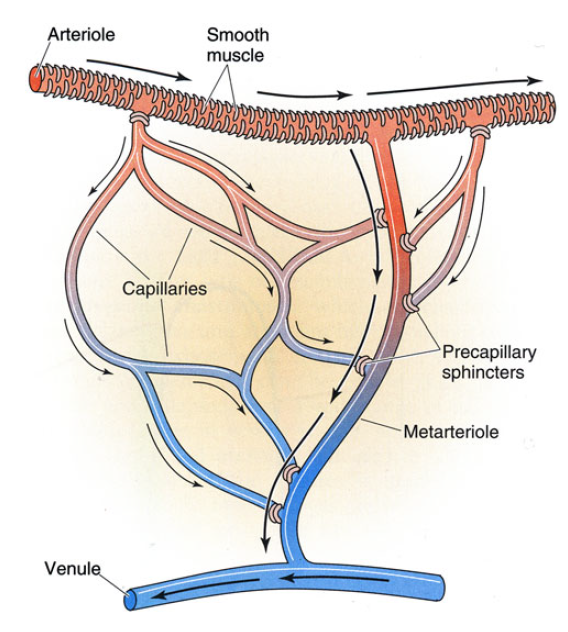
\includegraphics[width=.6\textwidth]{figures/capillary_bed}  
	\caption{something }
	\label{fig:beds}  
\end{figure}          

Each capillary entrance is controlled by a precapillary sphincter, which is composed of smooth muscle cells, that are able to contract or relax and thereby limit access of blood flow to certain capillaries.\cite{martini2012}

\subsection{Vasmotion}

The flow within the capillaries varies. This is due to the earlier mentioned precapillary sphincters contracts and relaxes     








